\documentclass[12pt]{article}

\usepackage{fullpage}
\usepackage{graphicx, rotating, booktabs} 
\usepackage{times} 
\usepackage{natbib} 
\usepackage{indentfirst} 
\usepackage{setspace}
\usepackage{grffile} 
\usepackage{hyperref}
\usepackage{adjustbox}
\usepackage{amsmath}
\usepackage{siunitx}
\usepackage{tikz} % for theoretical flow chart
\usetikzlibrary{shapes,decorations,arrows,calc,arrows.meta,fit,positioning}
\tikzset{
    -Latex,auto,node distance =1 cm and 1 cm,semithick,
    state/.style ={ellipse, draw, minimum width = 0.7 cm},
    point/.style = {circle, draw, inner sep=0.04cm,fill,node contents={}},
    bidirected/.style={Latex-Latex,dashed},
    el/.style = {inner sep=2pt, align=left, sloped}
}
\setcitestyle{aysep{}}


\singlespace
\title{\textbf{Sources of Alliance Treaty Depth}}
\author{Joshua Alley\footnote{Graduate Student,
Department of Political Science, Texas A\&M University.}}
\date{}

\bibliographystyle{apsr}

\begin{document}

\maketitle 

\doublespace 

\begin{abstract}
Why do states form deep alliances? 
Depth adds defense coordination and cooperation to promises of military support in alliances.
I argue that symmetric alliances between non-major powers are especially likely to include high treaty depth. 
In these alliances, members use treaty depth to support the implementation of unconditional military support and coordinate defense efforts. 
\end{abstract}


\newpage 


\section{Introduction}


% Start with hook: maybe a story of a deep and shallow alliance 
When do states form deep or shallow alliances? 
While some alliance treaties include only a promise of military support, others go beyond that by committing to extensive defense cooperation. 
For example, a 1962 alliance between Jordan and Saudi Arabia supplements defensive and offensive obligations with a planned military union and joint high command. 
Other alliances, such as a 1951 pact between the US and the Philippines, only include military support. 


There is substantial variation in how much depth states incorporate in their alliance treaties. 
As \autoref{fig:depth-motive} shows, many alliances have some depth. 
At least half of all ATOP alliances with offensive or defense obligations have at least one source of treaty depth.   
Moreover, the prevalence of deep alliances increased after 1945. 

\begin{figure}[hbtp]
\centering
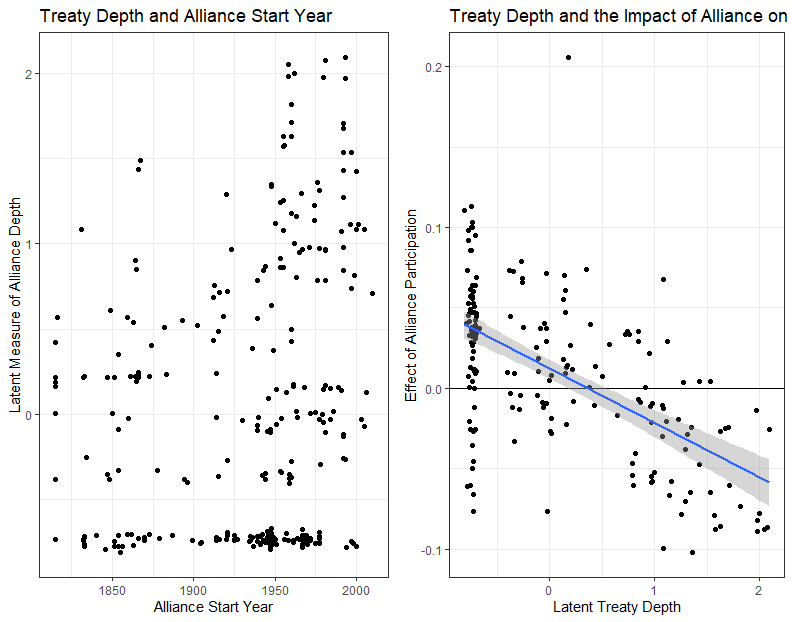
\includegraphics[width=0.95\textwidth]{../figures/depth-motive.png}
\caption{The left panel is a scatter plot of alliance treaty depth against the start year of the alliance. Each point marks an ATOP offensive or defensive alliance from 1815 to 2010. I created this measure of depth measure using a latent variable model. Values around -0.8 are alliances with no depth, so larger values imply the treaty has at least some depth. The right panel shows that the impact of alliance participation on non-major power military spending falls as treaty depth increases.}
\label{fig:depth-motive}
\end{figure}


% Deep alliances matter: affect milex, maybe credibility 
The institutional design choice to add formal treaty depth to an alliance has important consequences. 
Deep alliances encourage reduced military spending by non-major power members because treaty depth increases alliance credibility.  
The right panel of \autoref{fig:depth-motive} shows this relationship. 
Therefore, depth exerts a substantial impact on alliance politics by shaping treaty credibility and the distribution of military spending burdens among members. 


% Describe question and contribution of the paper
Despite the consequences of alliance treaty depth, we know fairly little about when states add depth to their alliances.\footnote{\citet{Mattes2012} examines a related measure of military institutionalization.}
In this paper, I explain when states form deep alliances, which clarifies when states design alliances that facilitate free-riding and require additional cooperation.  


% preview the argument 
My argument uses the alliance negotiation process to predict treaty depth. 
I argue that alliance member characteristics shape the obligations on military support in the treaty, which in turn affect the use of treaty depth. 
Alliance negotiations start by determining whether prospective members will offer military support and conditions on that support \citep{Poast2019a}. 
After establishing defensive or offensive support, alliance members negotiate over the use of treaty depth. 
In this process, alliance member characteristics shape the direct need for reassurance in this second stage, but also have an indirect effect on depth by affecting conditions on military support. 


Several alliance member characteristics could affect depth in this way, and I focus on symmetric alliances between non-major powers. 
Most studies of alliances examine famous alliances between major powers e.g. \citep{Snyder1997} or asymmetric treaties between major powers and non-major powers e.g. \citep{Morrow1991, Yarhi-Miloetal2016}. 
However, this approach pays little attention to the 42\% of ATOP military alliances that only involve non-major powers. % 122 / 289
After 1945, 60\% of all alliances are symmetric pacts between non-major powers. % 96 / 161
Thus, my argument elucidates dynamics within a large number of understudied alliances. 

% non-major power explains incidence of depth 
Symmetric alliances between non-major powers have greater depth than other alliances as depth is used to support promises of unconditional military support. 
Due to limited concern over entrapment and an emphasis on regional concerns, alliances between non-major powers are more likely to have unconditional military support. 
Non-major powers then add depth to these alliances to facilitate implementation of military support. % indirect effect  
Depth also helps non-major power allies maximize their limited coercive capacity, which establishes a direct path between non-major power alliances and depth. % direct effect


I test this argument with a series of statistical models and an illustrative case studies.
The statistical models employ multiple equations to approximate the alliance negotiation process. 
The case study checks the theoretical process and statistical results \citep{Seawright2016}.  


% roadmap for the paper 
The paper proceeds as follows. 
In the next section, I lay out the argument and hypothesis. 
Then I describe the data and research design 

\section{Argument}

In this argument, I start by defining treaty depth. 
Then, I briefly review existing work on alliance treaty design to establish that depth is under-studied. 
After that, I describe a general model of the process of alliance treaty negotiations. 
Finally, I describe how alliance negotiations between non-major powers tend to lead to higher treaty depth. 


% define alliance treaty depth
Alliance depth is the extent of defense cooperation formalized in the treaty. 
Deep alliances require additional military policy coordination and military cooperation. 
While shallow alliances stipulate more arms-length cooperation between members, deep treaties lead to closer cooperation through intermediate cooperation. 
Defense cooperation in a deep alliance takes many forms. 
Allies can form an integrated military command, provide military aid, commit to a common defense policy, provide basing rights, set up an international organization or undertake companion military agreements. 


% note that I'm the first one to address this question: lit review. 
Depth is therefore an important part of alliance treaty design. 
In general, alliances can be thought of as self-enforcing contracts or institutions \citep{Leedsetal2002, Morrow2000}.
Given external threats in an anarchic international system, states form treaties to aggregate military capability and secure their foreign policy interests \citep{Altfield1984, Smith1995, Snyder1997, FordhamPoast2014}. 


Potential alliance members can design a wide range of treaties \citep{Leedsetal2000, Leedsetal2002, Benson2012, BensonClinton2016}. 
Design considerations shape the costs and benefits of treaty participation. 
Beyond the benefit of potential military support, alliances also clarify international alignments \citep{Snyder1990}, support trade \citep{Gowa1995, Long2003, Fordham2010, WolfordKim2017}. 
The costs of alliances include lost foreign policy autonomy \citep{Altfield1984, Morrow2000, Johnson2015}, as well as the risk of opprtunistic behavior. 
Potential opportunism in alliances includes abandonment, or the failure of alliance members to honor their commitments \citep{BerkemeierFuhrmann2018}, entrapment in unwanted conflicts \citep{Snyder1984}, and free-riding \citep{Morrow2000}.  
Treaty design usually emphasizes the first two concerns as alliance members attempt to ensure the alliance is reliable and free from the risk of entrapment. 


% Depth is understudied
The process of alliance treaty design is understudied in general \citep{Poast2019a}. 
\citet{Mattes2012} offered an early study of alliance treaty design by using symmetry of capability and history of violation to explain conditionality, issue linkages, and military institutionalization in bilateral alliances. 
She argues that these three design considerations counter concerns about treaty reliability. 
\citet{Benson2012} shows that foreign policy disagreements and revisionist protege states increase the likelihood of limited military support commitments. 
\citep{Chibaetal2015} added to this by showing that democracies are more likely to form alliances with conditional military support or consultation. 
Other work by \citet{Poast2012, Poast2013} establishes that states often use issue linkages to facilitate alliance formation. 


None of these works directly study depth. 
\citet{Mattes2012} uses a similar measure of military institutionalization, but does not connect alliance conditionality with the use of depth. 
Rather, she treats depth and institutionalization as independent. 
Because states can use different foreign policy instruments as substitutes or complements \citep{Starr2000, MorganPalmer2000}, these different sources of reliability are probably related. 
My argument builds in part on \citet{Mattes2012}, but extends it by placing depth and conditions on military support in a unified theoretical and empirical framework. 
I now describe the general framework 

\subsection{Alliance Negotiations and Obligations}

% process of alliance negotiations: once agreed on military support, need to bolster. 
Observed alliance treaty designs are the outcome of negotiations between members \citep{Poast2019a}.  
Negotiation proceeds in two stages: first by determining the type of military support in the treaty, then by adding depth to the treaty as needed. 
Both stages address the benefits and costs of alliance participation, along with the risk of opportunism, each in different ways. 


% Part 1: Establish military support and conditions on that support
Establishing if and when military support will be offered is the primary task of potential alliance partners. 
Promises of military intervention are the essence of alliances. 
To form an alliance, the members must have sufficient overlap in foreign policy interests, especially their proposed war plans \citep{Morrow1991, Smith1995, FordhamPoast2014, Poast2019a}.  


Promises of military support in an alliance are not all or nothing, however. 
The extent of shared foreign policy interests shapes whether alliance members offer unconditional or conditional military support.
Many alliances limit promises of intervention to particular regions, conflicts, or instances of non-provocation \citep{Leedsetal2000}. 
For example, if alliance members fear entrapment in unwanted conflicts, they will only offer military support in specific circumstances \citep{Kim2011, Benson2012}.\footnote{Such deliberate design of alliances means clear instances of entrapment are rare \citep{Beckley2015}.} 
Conditional treaties reflect less overlap in foreign policy interests. 


On the other hand, offering unconditional military support is a strong signal of shared foreign policy interests. 
Attaching no conditions to a potential intervention means alliance members might hazard the reputational \citep{Gibler2008, Crescenzietal2012} and audience \citep{Fearon1997} costs of treaty violation in a variety of potential conflicts. 
Accepting these potential costs implies that conflict participation is acceptable; there is less fear of entrapment and many shared foreign policy interests. 
As a result, unconditional alliances are a key source of reliability. 


% Part 2: add depth as needed 
Having established parameters of military support, alliance partners then negotiate over how to reinforce those promises and put them into action. 
This second stage of the alliance negotiation is where alliance members determine the depth of the treaty. 
Depth shapes the perceived reliability of the treaty, by providing intermediate opportunities for states to fulfill treaty obligations in peacetime. 
Implementing costly depth-enhancing treaty provisions can also signal treaty credibility and enhance the ability of allies to fight together. 


Treaty depth depends on member characteristics and conditions on promises of military support from the first stage of the negotiations.
First, the presence of unconditional military support shapes formal treaty depth by increasing the need for policy coordination and intermediate signals of treaty reliability.\footnote{A counterargument is that states could use treaty depth to bolster the perceived reliability of conditional alliances.}
Time-inconsistency problems due to changing foreign policy interests are a major threat to alliance fulfillment 
\citep{LeedsSavun2007}. 
Although unconditional promises of military support are more credible, they are also more vulnerable to changing foreign policy interests. 
Under a deep alliance treaty, members can use implementation of defense cooperation and policy coordination to assess allied reliability. 


While alliance member characteristics shape conditions on military support, which then affect treaty depth, they also have a direct impact on treaty depth.  
Though states often make promises they intend to fulfill \citep{DownsRockeBarsoom1996, Chibaetal2015}, allies may still have greater reliability concerns with some states even after observing their promises of military support. 
This additional demand for reassurance increases the use of alliance treaty depth. 


\begin{figure}
\begin{center}
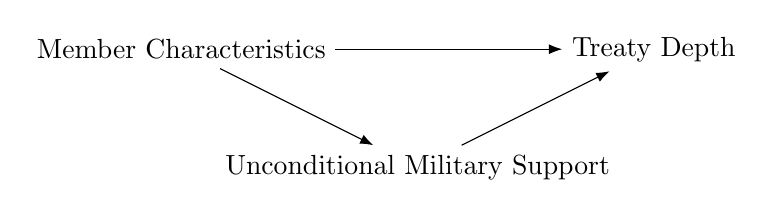
\begin{tikzpicture}[scale = 10]
    \node (1) at (0,0) {Member Characteristics};
    \node (2) at (.6,0)  {Treaty Depth}; %[right = of 1]
    \node (3) at(.3, -.15) {Unconditional Military Support};

    \path (1) edge (2);
    \path (1) edge (3);
    \path (3) edge (2);
\end{tikzpicture}
 \caption{General summary of the theoretical process. Alliance member characteristics affect treaty depth by changing the use of unconditional military support and directly changing the use of depth to boost treaty reliability.}
  \label{fig:theory-flow}
\end{center} 
\end{figure}


\autoref{fig:theory-flow} summarizes the process in the argument. 
Alliance member characteristics have a direct effect on treaty depth and an indirect effect through the use of unconditional military support. 
This pattern is especially clear for symmetric alliances between non-major powers, which tend to have higher depth. 


\subsection{Alliances between Non-major Powers}

% Move to process for non-major powers
Symmetry of capability in an alliance means all the members have roughly similar capabilities. 
Asymmetric alliances include both major and non-major powers, which generates an imbalance in military capabilities and foreign policy interests. 
Many of these treaties feature exchanges where the larger partner provides protection in exchange for foreign policy concessions \citep{Morrow1991, Johnson2015}. 
As such, alliance members often receive different foreign policy goods in asymmetric treaties. 


% aside on major powers: may cut that bit or footnote it
Unlike asymmetric alliances, symmetric pacts between states of similar capability share a common foreign policy goal or good.\footnote{Potential foreign policy goals include maintenance or change of the status quo \citep{MorganPalmer2006}.} 
Symmetric treaties between major powers are concerned with global balance of power \citep{Walt1990}, especially in multipolar international systems \citep{Snyder1984, Snyder1990, ChristensenSnyder1990}. 
These major power alliances are unlikely to include much depth, because substantial autonomy costs provide ample incentives for reliability, and very few major power alliances offer unconditional military support.


% Symmetric 
Alliance negotiations between non-major powers are more likely to produce alliances with substantial treaty depth. 
Non-major power treaties are more likely to include substantial depth because these alliances between non-major powers emphasize regional or local concerns.
Conversely, alliances with major power participation are linked with global concerns.
Though asymmetric alliances between major and non-major powers immediately address particular regional issues, they are part of major powers' expansive foreign policy concerns.  


% More unconditional alliances: less fear of entrapment w/ regional concerns
The limited scope of non-major power foreign policy ambitions attenuates concerns about entrapment. 
Where major powers are leery of being drawn into local conflicts, which increases their fear of entrapment.
Non-major power alliances often address these shared local conflicts. 
These alliances are often a form of local balancing, as they cannot usually offset a major power. 
Non-major powers also lack the power projection capabilities to entangle their partners in distant concerns. 
As a result, unconditional alliances between non-major powers still enhance credibility, but this obligation has different implications. 
Because there is less risk of entrapment in unwanted conflicts, non-major powers will be more likely to include unconditional military support in their alliances. 


% use depth to support joint war plans/policy coordination in uncond milsup
Their tendency to offer unconditional military support increases the depth of symmetric non-major power alliances. 
Depth backs unconditional military support by allowing alliance members to provide regular proof of their commitment to the alliance. 
Adding treaty depth also facilitates plans to provide military support in multiple contingencies.
Deep cooperation indicates that unconditional promises of military support are believable.  


% more depth due to potential efficiency gains
There is also a direct path between non-major power alliances and treaty depth. 
As non-major powers have more limited military capabilities, they may benefit more from policy coordination and defense cooperation. 
Deep alliances allow non-major powers to maximize the foreign policy benefits of their defense efforts. 
Rather than duplicate allied efforts, non-major powers can focus on particular issues.\footnote{Such policy coordination, coupled with the credibility from a combination of depth and unconditional military support, is the primary cause of free-riding in alliances by non-major powers.} 


Non-major powers' use of unconditional military support and desire to maximize their limited military resources both increase the depth of alliance treaties. 
Of these two mechanisms, the indirect path through unconditional military spending may be more important.
The sequence of alliance negotiations indicates that most of the effect of symmetric non-major power membership on treaty depth will operate through the establishment of unconditional military support. 


% brief illustration: Unconditional military support and policy coordination
% note that successful coord is not necessary, just thinking about design. 
% There are times when failure to implement deep promises is revelatory, which matches the argument. 
Many non-major power alliances combine unconditional military support and high treaty depth. 
For example, a 1976 alliance between Egypt and Sudan (ATOPID 3785) commits to unconditional military support, reinforced with a joint defense council and a joint staff command. 
This alliance grew out of shared regional concerns, especially disagreements with Libya. 
By promising to military support without restrictions on how or where the conflict began, Sudan and Libya increased their need for joint military planning. 
To give another example, many regional collective security organizations such as the African Union Common Defense and Security Pact (ATOPID 5055), also supplement unconditional defense promises with formal organizations and defense cooperation.  


An important caveat: this argument predicts institutional design, not implementation, let alone successful implementation. 
There are alliances where non-major power aspirations in alliance design are not fully realized, or work poorly. 
To give one example, several deep Pan-Arab alliances never realized their full intention due to internal political divisions.  


Based on the argument and these cases, I expect that alliance negotiations between non-major powers will produce deeper alliance treaties. 
The main mechanism behind this relationship is the use of unconditional military support, because treaty depth supports unconditional obligations. 
Non-major powers also use depth to maximize their limited military capabilities. 
In the next section, I describe how I will test this claim about the association between non-major power membership and treaty depth. 






\section{Research Design}



\section{Results}


\section{Conclusion}




\singlespace
 
\bibliography{../../../MasterBibliography} 





\end{document}